\section{Tecnologías}
Para el desarrollo del proyecto se propone utilizar las siguientes tecnologías que permitirán lograr los objetivos propuestos en el sistema. Las ventajas que representan para el desarrollo son descritas a continuación.
\vspace{10mm}
	\begin{table}[b!]
    \centering
    \vspace{-30mm}
      \begin{tabular}{|p{2cm}|ll}
        \hline
        
        \multicolumn{2}{|c|}{{\bf Cuadro comparativo de tecnologías}} \\ 
        \hline
          \multicolumn{1}{|p{4cm}|}{{\bf Nombre}} & 
		  \multicolumn{1}{p{10cm}|}{{\bf Características}}\\

        \hline
          \multicolumn{1}{|p{5cm}|}{Base de datos relacional} & 
          \multicolumn{2}{p{10cm}|}{\begin{itemize}
          \vspace{-5mm}
        \item Es un tipo de base de datos que cumple con el modelo relacional.
        \item Permite establecer interconexiones o relaciones entre los datos,y a través de dichas conexiones relacionar los datos de ambas tablas, de ahí proviene su nombre: "modelo relacional".
        \item No pueden existir dos tablas con el mismo nombre ni registro.
        \item Cada tabla es a su vez un conjunto de campos (columnas) y registros (filas).
        \item Las claves primarias son la clave principal de un registro dentro de una tabla y estas deben cumplir con la integridad de datos.
       
      \end{itemize}} \\
         
        \hline
          \multicolumn{1}{|p{5cm}|}{Bases de datos no relacional} & 
          \multicolumn{1}{p{10cm}|}{
          \begin{itemize}
          \vspace{-5mm}
          \item Los datos almacenados no requieren estructuras fijas como tablas, normalmente no soportan operaciones JOIN.
        \item Pueden manejar enormes cantidades de datos.
        \item No generan cuellos de botella.
        \item Escalamiento sencillo.
        \item Se ejecutan en clusters de máquinas baratas.
        \item No usan SQL como el principal lenguaje de consultas
      \end{itemize}} \\ 
       \hline
        
      \end{tabular}
     
      \label{Cuadro Comparativo}
    \end{table}
\newpage
	\begin{table}[b!]
    \centering
    \vspace{-5mm}
      \begin{tabular}{|p{2cm}|ll}
        \hline
        
          \multicolumn{1}{|p{5cm}|}{Base de datos Orientada a grafos} & 
          \multicolumn{2}{p{10cm}|}{\begin{itemize}
          \vspace{-5mm}
        \item Representa la información como nodos de un grafo y sus relaciones con las aristas del mismo
        \item Consultas más amplias y no demarcadas por tablas.
        \item No hay que definir un número determinado de atributos.
        \item Los registros también son de longitud variable, evitando tener que definir un tamaño y también posibles fallas en la base de datos.
        \item Se puede recorrer directamente la base de datos de forma jerárquica, obtener el nodo abuelo del nodo y viceversa.
      \end{itemize}} \\
       \hline
       
      \end{tabular}
      \caption{Tipos de bases de datos}
      \label{Cuadro comparativo}
    \end{table}
    
\newpage

	\begin{table}[b!]
    \centering
      \begin{tabular}{|p{2cm}|ll}
        \hline
        \multicolumn{2}{|c|}{{\bf Cuadro comparativo de tecnologías}} \\ 
        \hline
          \multicolumn{1}{|p{4cm}|}{{\bf Nombre}} & 
		  \multicolumn{1}{p{10cm}|}{{\bf Características}}\\

        \hline
          \multicolumn{1}{|p{5cm}|}{
\includegraphics[width=0.3\textwidth]{images/neo4j}} & 
          \multicolumn{2}{p{10cm}|}{\begin{itemize}
          \vspace{-15mm}
        \item Es una base de datos open-source,esta escrita en java.
        \item Permite realizar transacciones ACID.
        \item Manera su propio lenguaje de query , Cypher.
        \item Puede contener billiones de nodos y relaciones.
        \item Rápido recorriendo relaciones, este tipo de queries se conoce como transversals
        \item Las escrituras se pueden realizar en cualquier instancia del clúster.
        \item Multilenguaje, proporciona una Api Rest pudiendo utilizarse desde cualquier lenguaje.
      \end{itemize}} \\
         
        \hline
          \multicolumn{1}{|p{5cm}|}{
\includegraphics[width=0.3\textwidth]{images/InfiniteGraph}} & 
          \multicolumn{1}{p{10cm}|}{
          \begin{itemize}
          \vspace{-7mm}
        \item Posee almacenamiento en la nube.
        \item Apoyo de consultas en paralelo.
        \item Precios felixibles y opciones de licencia.
        \item Totalmente transaccional y multi-hilo.
      \end{itemize}} \\ 
        \hline
          \multicolumn{1}{|p{3cm}|}{
\includegraphics[width=0.3\textwidth]{images/InfoGrid}} & 
          \multicolumn{1}{p{10cm}|}{
          \begin{itemize}
          \vspace{-10mm}
        \item Recorrido Gráfico y consultas de tipo relacional.
        \item Indexación personalizable.
        \item Gestión de almacenamiento personalizable.
      \end{itemize}}\\ 
         \hline
        %\hline
      \end{tabular}
      \caption{Cuadro comparativo de gestores de bases de datos orientadas a grafos}
      \label{table:bd orientadas a grafos}
    \end{table}
\newpage
\begin{table}[b!]
    \centering
      \begin{tabular}{|p{1cm}|l}
        \hline
        \multicolumn{2}{|c|}{{\bf Cuadro comparativo de tecnologías}} \\ 
        \hline
          \multicolumn{1}{|p{4cm}|}{{\bf Nombre}} & 
		  \multicolumn{1}{p{10cm}|}{{\bf Características}}\\
		 \hline
          \multicolumn{1}{|p{5cm}|}{
\includegraphics[width=0.3\textwidth]{images/bootstrap}} & 
          \multicolumn{1}{p{10cm}|}{\begin{itemize} 
       \vspace{-20mm}
          \item Es un framework o conjunto de herramientas de software libre para diseño de sitios y aplicaciones web. 
        \item Contiene plantillas de diseño con tipografía, formularios, botones, cuadros, menús de navegación y otros elementos de diseño basado en HTML y CSS, así como, extensiones de JavaScript opcionales adicionales.
        \item Es compatible con la mayoría de los navegadores web.
        \item Bootstrap es de código abierto y está disponible en GitHub. 
        \item Desde la versión 2.0 también soporta diseños sensibles. Esto significa que el diseño gráfico de la página se ajusta dinámicamente, tomando en cuenta las características del dispositivo usado (Computadoras, tabletas, teléfonos móviles).
      \end{itemize}} \\
         
        \hline
          \multicolumn{1}{|p{5cm}|}{
\includegraphics[width=0.3\textwidth]{images/foundation}} & 
          \multicolumn{1}{p{10cm}|}{ 
          \begin{itemize}
                 \vspace{-20mm}
          \setlist[itemize]{noitemsep, topsep=0pt}  
          	\item No tiene que agregar clases de responder o lograr cierto estilo.
			\item Muchos prefieren Foundation, ya que ofrece más flexibilidad.
			\item Fácil navegación de su sitio a otro sitio.
            \item Tablas de precios,diseñado para mostrar los precios de un producto a base de suscripción
            \item Las páginas web se ajustan a diferentes dispositivos.
         \end{itemize}}\\ 
        \hline
        %\hline
      \end{tabular}
      \caption{Cuadro de tecnologías para diseño Web}
      \label{table:tecnologias web}
    \end{table}
\newpage
\begin{table}[b!]
    \centering
    \vspace{-30mm}
      \begin{tabular}{|p{2cm}|ll}
        \hline
        
        \multicolumn{2}{|c|}{{\bf Cuadro comparativo de tecnologías}} \\ 
        \hline
          \multicolumn{1}{|p{4cm}|}{{\bf Nombre}} & 
		  \multicolumn{1}{p{10cm}|}{{\bf Características}}\\

        \hline
          \multicolumn{1}{|p{5cm}|}{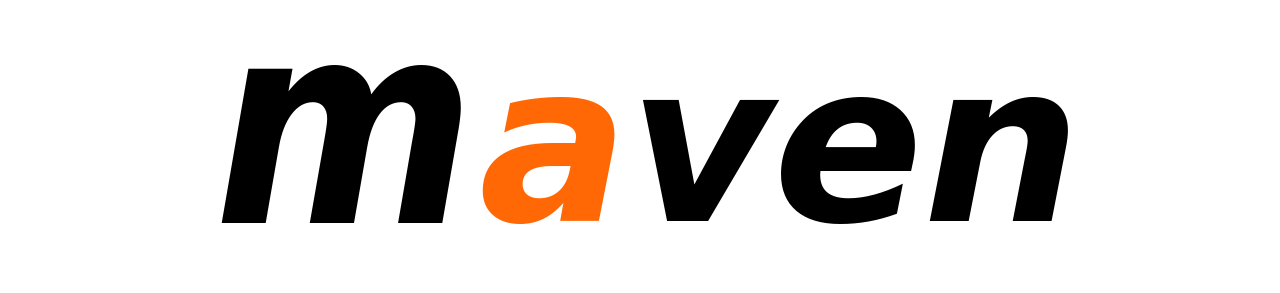
\includegraphics[width=0.3\textwidth]{images/maven}} & 
          \multicolumn{2}{p{10cm}|}{\begin{itemize}
          \vspace{-10mm}
        \item Es una herramienta de software para la gestión y construcción de proyectos.
        \item Tiene un modelo de configuración de construcción más simple, basado en un formato XML.
        \item Utiliza un Project Object Model (POM) para describir el proyecto de software a construir, sus dependencias de otros 				módulos y componentes externos, y el orden de construcción de los elementos.
        \item  Viene con objetivos predefinidos para realizar ciertas tareas claramente definidas, como la compilación del código y su 		empaquetado.
        \item El motor incluido en su núcleo puede dinámicamente descargar plugins de un repositorio.
        \item Está construido usando una arquitectura basada en plugins que permite que utilice cualquier aplicación controlable a través de la entrada estándar. 
       
      \end{itemize}} \\
         
        \hline
          \multicolumn{1}{|p{5cm}|}{
\includegraphics[width=0.3\textwidth]{images/ant}} & 
          \multicolumn{1}{p{10cm}|}{
          \begin{itemize}
          \vspace{-27mm}
          \item Es una herramienta usada en programación para la realización de tareas mecánicas y repetitivas, normalmente durante la fase de compilación y construcción (build). 
        \item Es un software para procesos de automatización de compilación, similar a Make pero desarrollado en lenguaje Java y requiere la plataforma Java, así que es más apropiado para la construcción de proyectos Java.
        \item Esta herramienta, hecha Java, tiene la ventaja de no depender de las órdenes del shell de cada sistema operativo, sino que se basa en archivos de configuración XML 
        \item  Ant utiliza XML para describir el proceso de generación y sus dependencias.
      
      \end{itemize}} \\ 
       \hline
        
      \end{tabular}
     
      \label{Cuadro Comparativo}
    \end{table}
